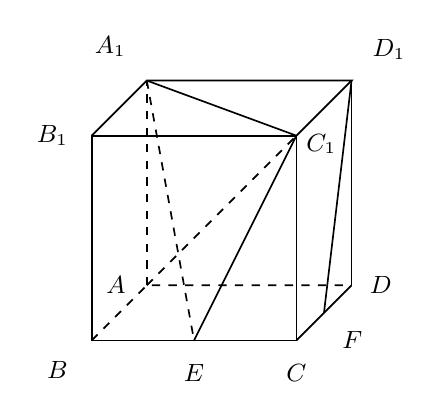
\begin{tikzpicture}[line width=.6pt,font=\small]
\coordinate (B) at (0,0);
\coordinate (E) at (1.3,0);
\coordinate (C) at (2.6,0);
\coordinate (F) at (2.9500000000,0.3500000000);
\coordinate (D) at (3.3,0.7);
\coordinate (A) at (0.7,0.7);
\coordinate (B1) at (0,2.6);
\coordinate (C1) at (2.6,2.6);
\coordinate (D1) at (3.3,3.3);
\coordinate (A1) at (0.7,3.3);
\draw (B) -- (E) -- (C) -- (C1) -- (B1) -- cycle;

\draw (C) -- (F) -- (D);
\draw (C1) -- (D1) -- (A1) -- (B1);

\draw (A1) -- (C1);
\draw (E) -- (C1);
\draw (D1) -- (F);
\draw (D1) -- (D);
\draw[dashed] (B) -- (A) -- (D);
\draw[dashed] (A) -- (A1);
\draw[dashed] (A) -- (C1);
\draw[dashed] (A1) -- (E);
\node[below left,xshift=-5pt,yshift=-4pt] at (B) {$B$};
\node[below,yshift=-5pt] at (E) {$E$};
\node[below,yshift=-5pt] at (C) {$C$};
\node[below right=3pt] at (F) {$F$};
\node[right=3pt] at (D) {$D$};
\node[left,xshift=-4pt,yshift=0pt] at (A) {$A$};
\node[left,xshift=-5pt] at (B1) {$B_{1}$};
\node[right,xshift=0pt,yshift=-3pt] at (C1) {$C_{1}$};
\node[above right,xshift=4pt,yshift=4pt] at (D1) {$D_{1}$};
\node[above left,xshift=-4pt,yshift=5pt] at (A1) {$A_{1}$};
\end{tikzpicture}
